\documentclass[12pt]{article}

\usepackage[margin=1in]{geometry}
\usepackage{fancyhdr}
\usepackage{amsmath, amsfonts, amsthm, amssymb, mathtools}  % Some math symbols
\usepackage{color}
% \usepackage{sectsty}
\usepackage{tcolorbox}
\usepackage{amsfonts}
\usepackage{titletoc}
\usepackage{caption}
\usepackage[normalem]{ulem}
\usepackage{graphicx}


\usepackage{hyperref}
\hypersetup{
    colorlinks,
    citecolor=black,
    filecolor=black,
    linkcolor=black,
    urlcolor=black
}


\titlecontents{section}[0em]
{\smallskip}
{\thecontentslabel\enspace}
{\hspace*{-5.3em}}
{\hfill\contentspage}



%%%%%%%%%%%% SETUP %%%%%%%%%%%%

% name of the class
\newcommand{\classname}{CSE 371}
% name of the assignment
\newcommand{\assignmentname}{HW4}
% collaborators on assignment
\newcommand{\collaborators}{Cameron Jennings (ID: 2029631), Donovan Clay (ID: 2276005)}
\newcommand{\listcollaborators}{Collaborators: \collaborators}

\pagestyle{fancy}
\fancyhf{}
\setlength{\headheight}{13.59999pt}
\rhead{\thepage}
\lhead{\hyperref[beginning]{\classname \hspace{1em} \assignmentname}}

\usepackage{titlesec}
\titleformat{\subsection}{\normalfont\fontsize{12}{15}\bfseries}{\thesubsection}{1em}{}

\titleformat{\section}[block]
{\filcenter\large
\addtolength{\titlewidth}{2pc}%
\titleline*[c]{}%
\addvspace{6pt}%
}
{\thesection}{1em}{}
\titlespacing{\section}
{5pc}{*2}{*2}[5pc]


% \definecolor{WordSectionBlue}{RGB}{30, 90, 147}
% \allsectionsfont{\color{WordSectionBlue}}

%%%%%%%%%%%% FILE SPECIFIC IMPORTS %%%%%%%%%%%%

\usepackage{ragged2e}
\usepackage{tikz}

%%%%%%%%%%%%%%%%%%%%%%%%%%%%%%%%%%%%%%%%%%%%%%%

\renewcommand*{\thesection}{Question \arabic{section}.}
\renewcommand{\thesubsection}{(\alph{subsection})}

%%%%%%%%%%%% ENVIRONMENTS %%%%%%%%%%%%

\newenvironment{explanation}{\begin{tcolorbox}[colback=blue!2!white,colframe=blue!20!white]}{\end{tcolorbox}}

\newenvironment{subquestion}[1]{\subsection{#1}
\begin{tcolorbox}[colback=blue!2!white,colframe=blue!20!white]}{\end{tcolorbox}}

\newenvironment{sssq}[3]{\textbf{\thesubsubsection.\sssqARG{#1}} \hspace{0.5cm}
\begin{minipage}[t][\sssqARG{#2}][t]{14cm}
    \textbf{\sssqARG{#3}}
\end{minipage}
\begin{explanation}
}{\end{explanation}}

%%%%%%%%%%%% MY MACROS %%%%%%%%%%%%

\newcommand{\prob}{\mathbb{P}}
\newcommand{\expect}{\mathbb{E}}
\newcommand*\sssqARG{}
\newcommand{\bayes}{\textbf{Bayes' Theorem}}
\newcommand{\ltp}{\textbf{Law of Total Probability}}
\newcommand{\var}{\text{Var}}
\newcommand{\unif}{\sim \text{Unif}}
\newcommand{\expo}{\sim \text{Exponential}}
\newcommand{\caseif}{\text{if }}
\newcommand{\nlog}{\text{ln}}


%%%%%%%%%%%%%%%%%%%%%%%%%%%%%%%%%%%%%%
\begin{document}

    \setcounter{tocdepth}{1}
    \begin{center}\label{beginning}
        \tableofcontents 
    \end{center}

    \begin{center}
        \listcollaborators
    \end{center}

    % fix section heading font
    \titleformat{\section}{\normalfont\fontsize{17.28}{15}\bfseries\raggedright}{\thesection}{1em}{}
    \newpage
    \AddToHook{cmd/section/before}{\clearpage}

    % Question 1
    \section{Draw the ASMD chart for each of the following state transition description.}
        \begin{subquestion}{}
            \begin{center}
                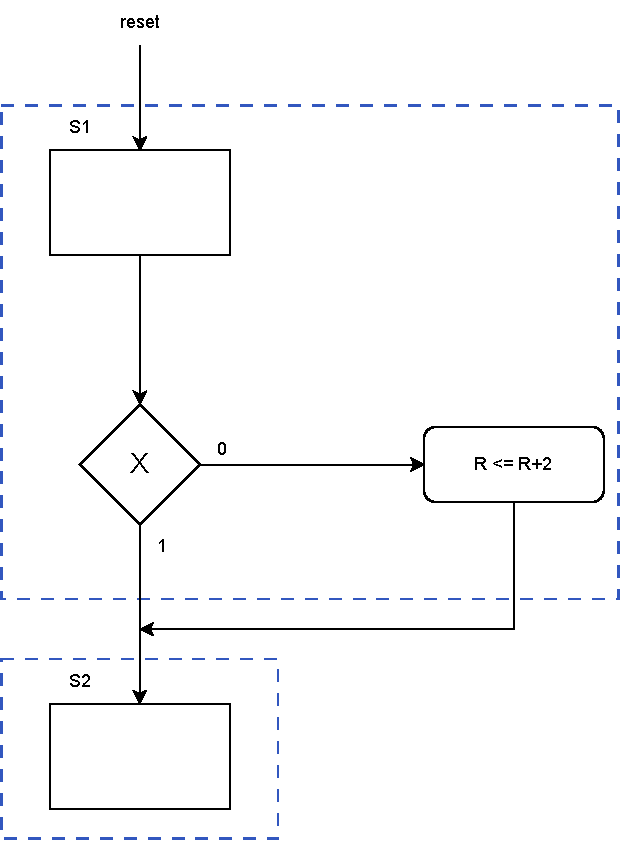
\includegraphics[scale=0.5]{Images/Question 1a.pdf}
            \end{center}
        \end{subquestion}

        \begin{subquestion}{}
            \begin{center}
                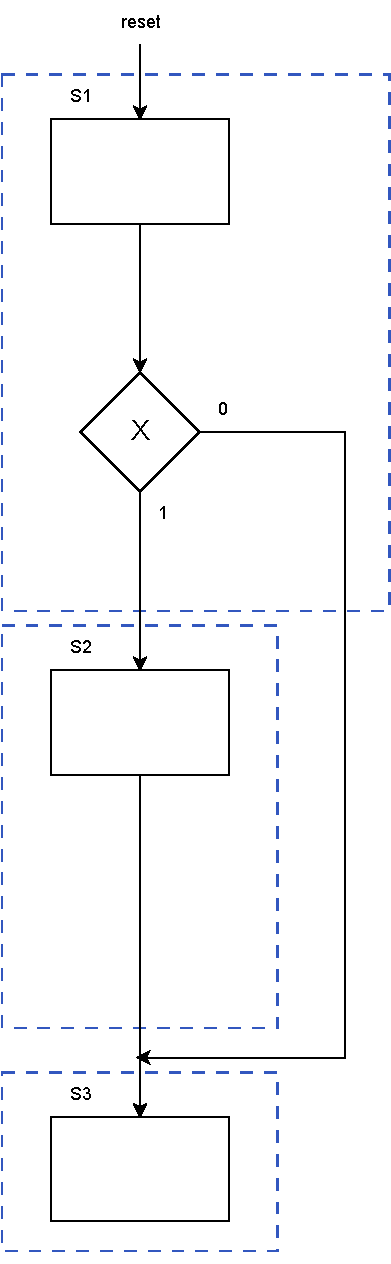
\includegraphics[scale=0.5]{Images/Question 1b.pdf}
            \end{center}
        \end{subquestion}

        \begin{subquestion}{}
            \begin{center}
                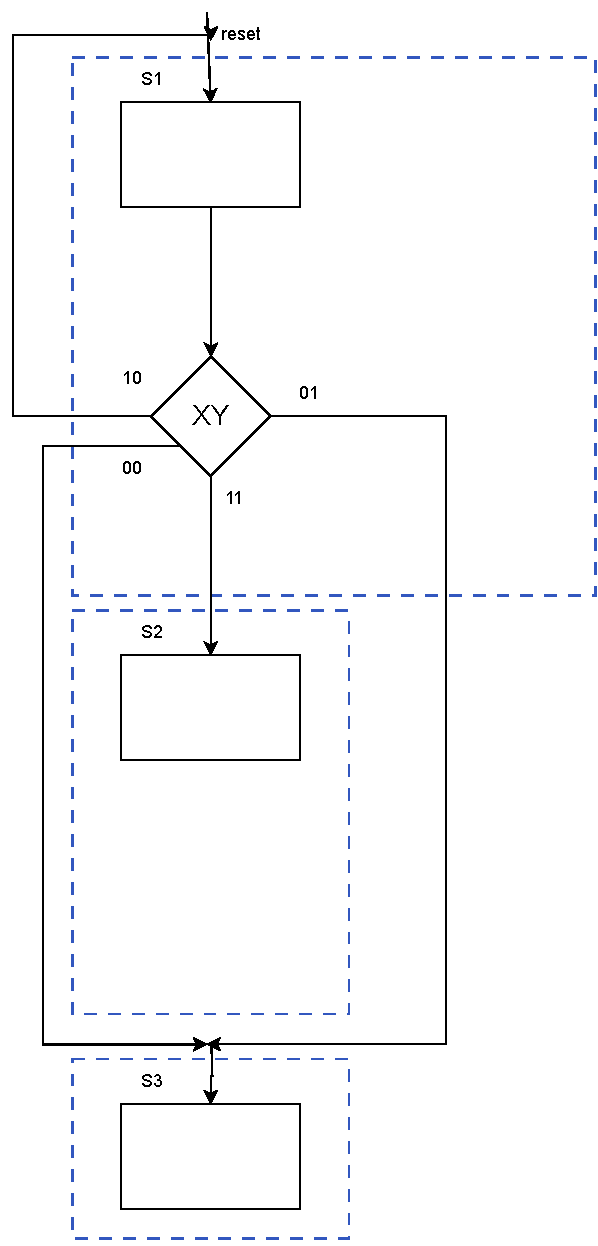
\includegraphics[scale=0.5]{Images/Question 1c.pdf}
            \end{center}
        \end{subquestion}
        

    % Question 2
    \section{}
        \begin{explanation}
            \begin{center}
                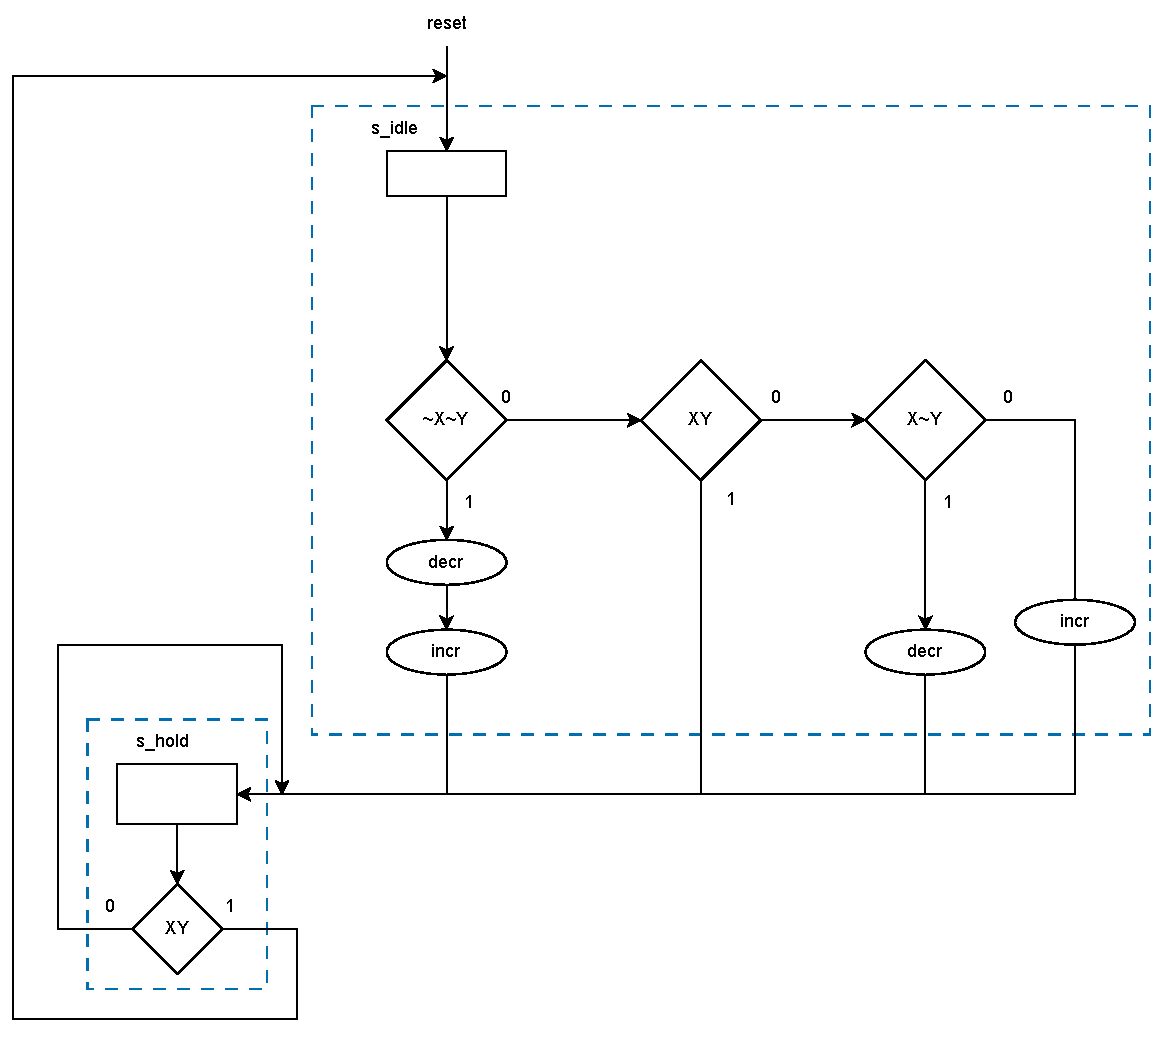
\includegraphics[scale=0.7]{Images/Question 2 second try.pdf}
            \end{center}
            \begin{center}
                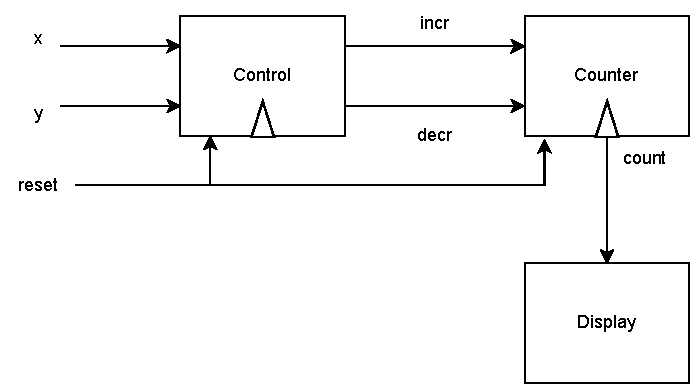
\includegraphics[scale=1]{Images/Question 2 datapath circuit.pdf}
            \end{center}
        \end{explanation}
        
        
        
    % Question 3
    \section{}
        \begin{explanation}
            Testbench before:
            \begin{center}
                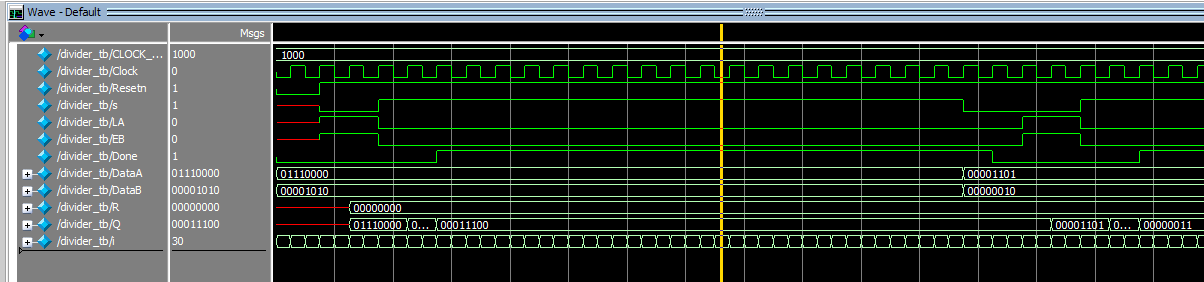
\includegraphics[scale = 0.47]{Images/before.PNG}
            \end{center}
            This testbench shows that the Q is getting right hifted instead of getting left shifted into R. Second, the down counter starts at 0 and never changes. And that makes it so R is never updated.

            Testbench after:
            \begin{center}
                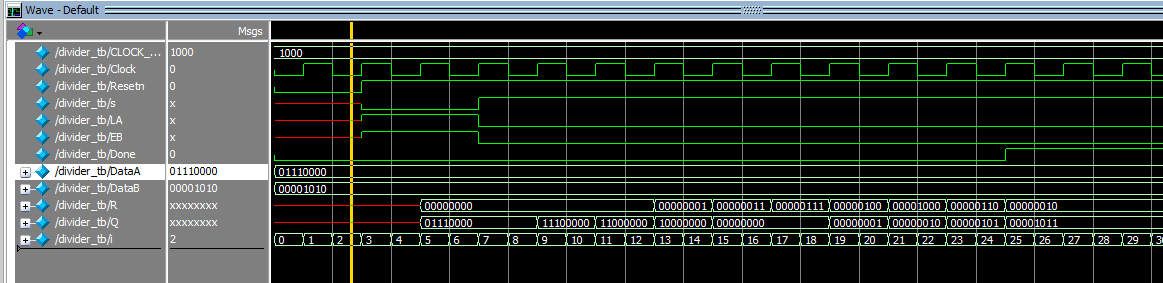
\includegraphics[scale = 0.5]{Images/after.PNG}
            \end{center}
        \end{explanation}

        
        

    \section{Experience Report}
        We found this homework to be medium. Problem 3 was definitely the most confusing part because we had to figure the starter code and understanding that took the most time. 
        \begin{description}
            \item[Question 1:] 30 minutes
            \item[Question 2:] 1.5 hours
            \item[Question 3:] 3 hours
        \end{description}        
\end{document}
